%%%%%%%%%%%%%%%%%%%%%%%%%%%%%%%%%%%%%%%%%
% mainpage.tex v3.0
%
% Relazione per il progetto PuzzleSolver (Parte 3)
% Autore: Giacomo Cusinato
% Materia: Programmazione Concorrente e Distribuita
%
% This document is based on Simple Sectioned Essay template:
% http://www.latextemplates.com/template/simple-sectioned-essay
%
%%%%%%%%%%%%%%%%%%%%%%%%%%

%----------------------------------------------------------------------------------------
%	PACKAGES AND OTHER DOCUMENT CONFIGURATIONS
%----------------------------------------------------------------------------------------

\documentclass[12pt]{article} % Default font size is 12pt, it can be changed here

\usepackage{geometry} % Required to change the page size to A4
\geometry{a4paper} % Set the page size to be A4 as opposed to the default US Letter

\usepackage[italian]{babel}
\usepackage[utf8]{inputenc}

\usepackage{graphicx} % Required for including pictures

\usepackage{float} % Allows putting an [H] in \begin{figure} to specify the exact location of the figure
\usepackage{wrapfig} % Allows in-line images such as the example fish picture

\usepackage{lipsum} % Used for inserting dummy 'Lorem ipsum' text into the template

\usepackage{verbatim} % for multiline comments
\usepackage{caption}

\usepackage{url} % Allows using urls


\linespread{1.2} % Line spacing

\begin{document}

	%----------------------------------------------------------------------------------------
	%	TITLE PAGE
	%----------------------------------------------------------------------------------------

	\begin{titlepage}

		\newcommand{\HRule}{\rule{\linewidth}{0.5mm}} % Defines a new command for the horizontal lines, change thickness here

		\center % Center everything on the page

		\textsc{\LARGE Università degli Studi di Padova}\\[1.5cm] % Name of your university/college
		\textsc{\Large Programmazione Concorrente e Distribuita}\\[0.5cm] % Major heading such as course name
		\textsc{\large A.A. 2014/2015}\\[0.5cm] % Minor heading such as course title

		\HRule \\[0.8cm]
		{ \huge \bfseries Risolutore di Puzzle - Parte 3}\\[0.4cm] % Title of your document
		\HRule \\[1.5cm]


		Autore: \\[\baselineskip]
		{\Large GIACOMO CUSINATO }\\
		{\large \emph{Mat.} 1054137 }\\[4cm] % Editor list

		{\large \today}\\[3cm] % Date, change the \today to a set date if you want to be precise

		\vfill % Fill the rest of the page with whitespace

	\end{titlepage}

	%----------------------------------------------------------------------------------------
	%	TABLE OF CONTENTS
	%----------------------------------------------------------------------------------------

	\tableofcontents % Include a table of contents

	\newpage % Begins the essay on a new page instead of on the same page as the table of contents

	%----------------------------------------------------------------------------------------
	%	ABSTRACT
	%----------------------------------------------------------------------------------------

	%%%%%%%%%%%%%%%%%%%%%%%%%%%%%%%%%%%%%%%%%
% ambiente_di_sviluppo.tex v1.0
%
% Relazione per il progetto PuzzleSolver (Parte 1)
% Autore: Giacomo Cusinato
% Materia: Programmazione Concorrente e Distribuita
%
% This document is based on Simple Sectioned Essay template:
% http://www.latextemplates.com/template/simple-sectioned-essay
%
%%%%%%%%%%%%%%%%%%%%%%%%%%		

\section{Ambiente di sviluppo}
Il progetto \`{e} stato realizzato principalmente in ambiente Windows (nello specifico Windows 8.1 Pro 64bit) tramite l'uso dell'IDE Intellij IDEA \url{https://www.jetbrains.com/idea/}. \`{E} stato inoltre testato con successo nella macchine di laboratorio con i dovuti comandi per impostare Java 7 come versione principale del sistema.
Per la stesura della relazione, invece, \`{e} stato utilizzato il linguaggio \LaTeX{} in ambiente Mac OS X (Yosemite 10.10) tramite la ditribuzione MacTex.
Nel progetto, come richiesto, \`{e} stato incluso un makefile per semplificare la complilazione dei sorgenti. 

	%%%%%%%%%%%%%%%%%%%%%%%%%%%%%%%%%%%%%%%%%
% differenze_con_la_versione_precedente.tex v2.0
%
% Relazione per il progetto PuzzleSolver (Parte 3)
% Autore: Giacomo Cusinato
% Materia: Programmazione Concorrente e Distribuita
%
%%%%%%%%%%%%%%%%%%%%%%%%%%%%%%%%%%%%%%%%%

\section{Differenze con la versione precedente}

Come da specifica, il progetto è stato suddiviso in modo tale da simulare l'interazione tra un client ed un server
tramite tecnologia RMI. Tutta la logica e le classi relative ala risoluzione del puzzle sono state spostate nella
parte server, in quanto il client si occuperà esclusivamente delle operazioni input/output ottenendo il risultato
finale tramite una chiamata al metodo \texttt{reoder(String inputContent)} definito nell'oggetto remoto.

\subsection{Classi lato server}

Di seguito le classi che definiscono il modulo server del progetto:

\begin{itemize}
    \item \texttt{Block}: rappresenta una tessera del puzzle. Rimane invariata rispetto alle precedenti consegne ma
    fa ora parte del modulo server.
    \item \texttt{PuzzleThread}: La classe PuzzleThread definisce un un oggetto la cui istanza può essere lanciata
    dal programma in un thread a supporto della risoluzione dell’algorimo. Anche questa classe rimane invarita
    rispetto alla precedente consegna ed è stata inserita nel modulo server.
    \item \texttt{PuzzleSolverServer}: è la classe principale del modulo server. Contiene la logica dell'algoritmo di
    risoluzione del puzzle (rimasta invariata) ed espone il metodo \texttt{reoder(String inputContent)} che può essere
    invocato da una JVM remota e restituisce la soluzione prodotta. Il metodo \texttt{main} crea un'istanza di questa
    classe e ne registra il riferimento nel registro RMI.
\end{itemize}


\subsection{Classi lato client}

Di seguito le classi che definiscono il modulo client del progetto:

\begin{itemize}
    \item \texttt{IOHelper}: si occupa di effettura la lettura e la scrittura di stringhe su determinati file.
    Questa classe è rimasta invariata rispetto alle consegne precedenti.
    \item \texttt{PuzzleSolverClient}: è la casse principale del modulo client. Oltre a sfruttare i metodi esposti
    dalla classe \texttt{IOHelper}, si occupa di ottenere il riferimento all'oggetto remoto e chiamare il metodo
    \texttt{reoder(String inputContent)} così da ottenere la soluzione del puzzle tramite il server.
\end{itemize}

	%%%%%%%%%%%%%%%%%%%%%%%%%%%%%%%%%%%%%%%%%
% implementazione_del_sistema_rmi.tex v1.0
%
% Relazione per il progetto PuzzleSolver (Parte 3)
% Autore: Giacomo Cusinato
% Materia: Programmazione Concorrente e Distribuita
%
%%%%%%%%%%%%%%%%%%%%%%%%%%%%%%%%%%%%%%%%%

\section{Implementazione del sistema RMI}

\begin{figure}[htbp]
    \centering
    \centerline{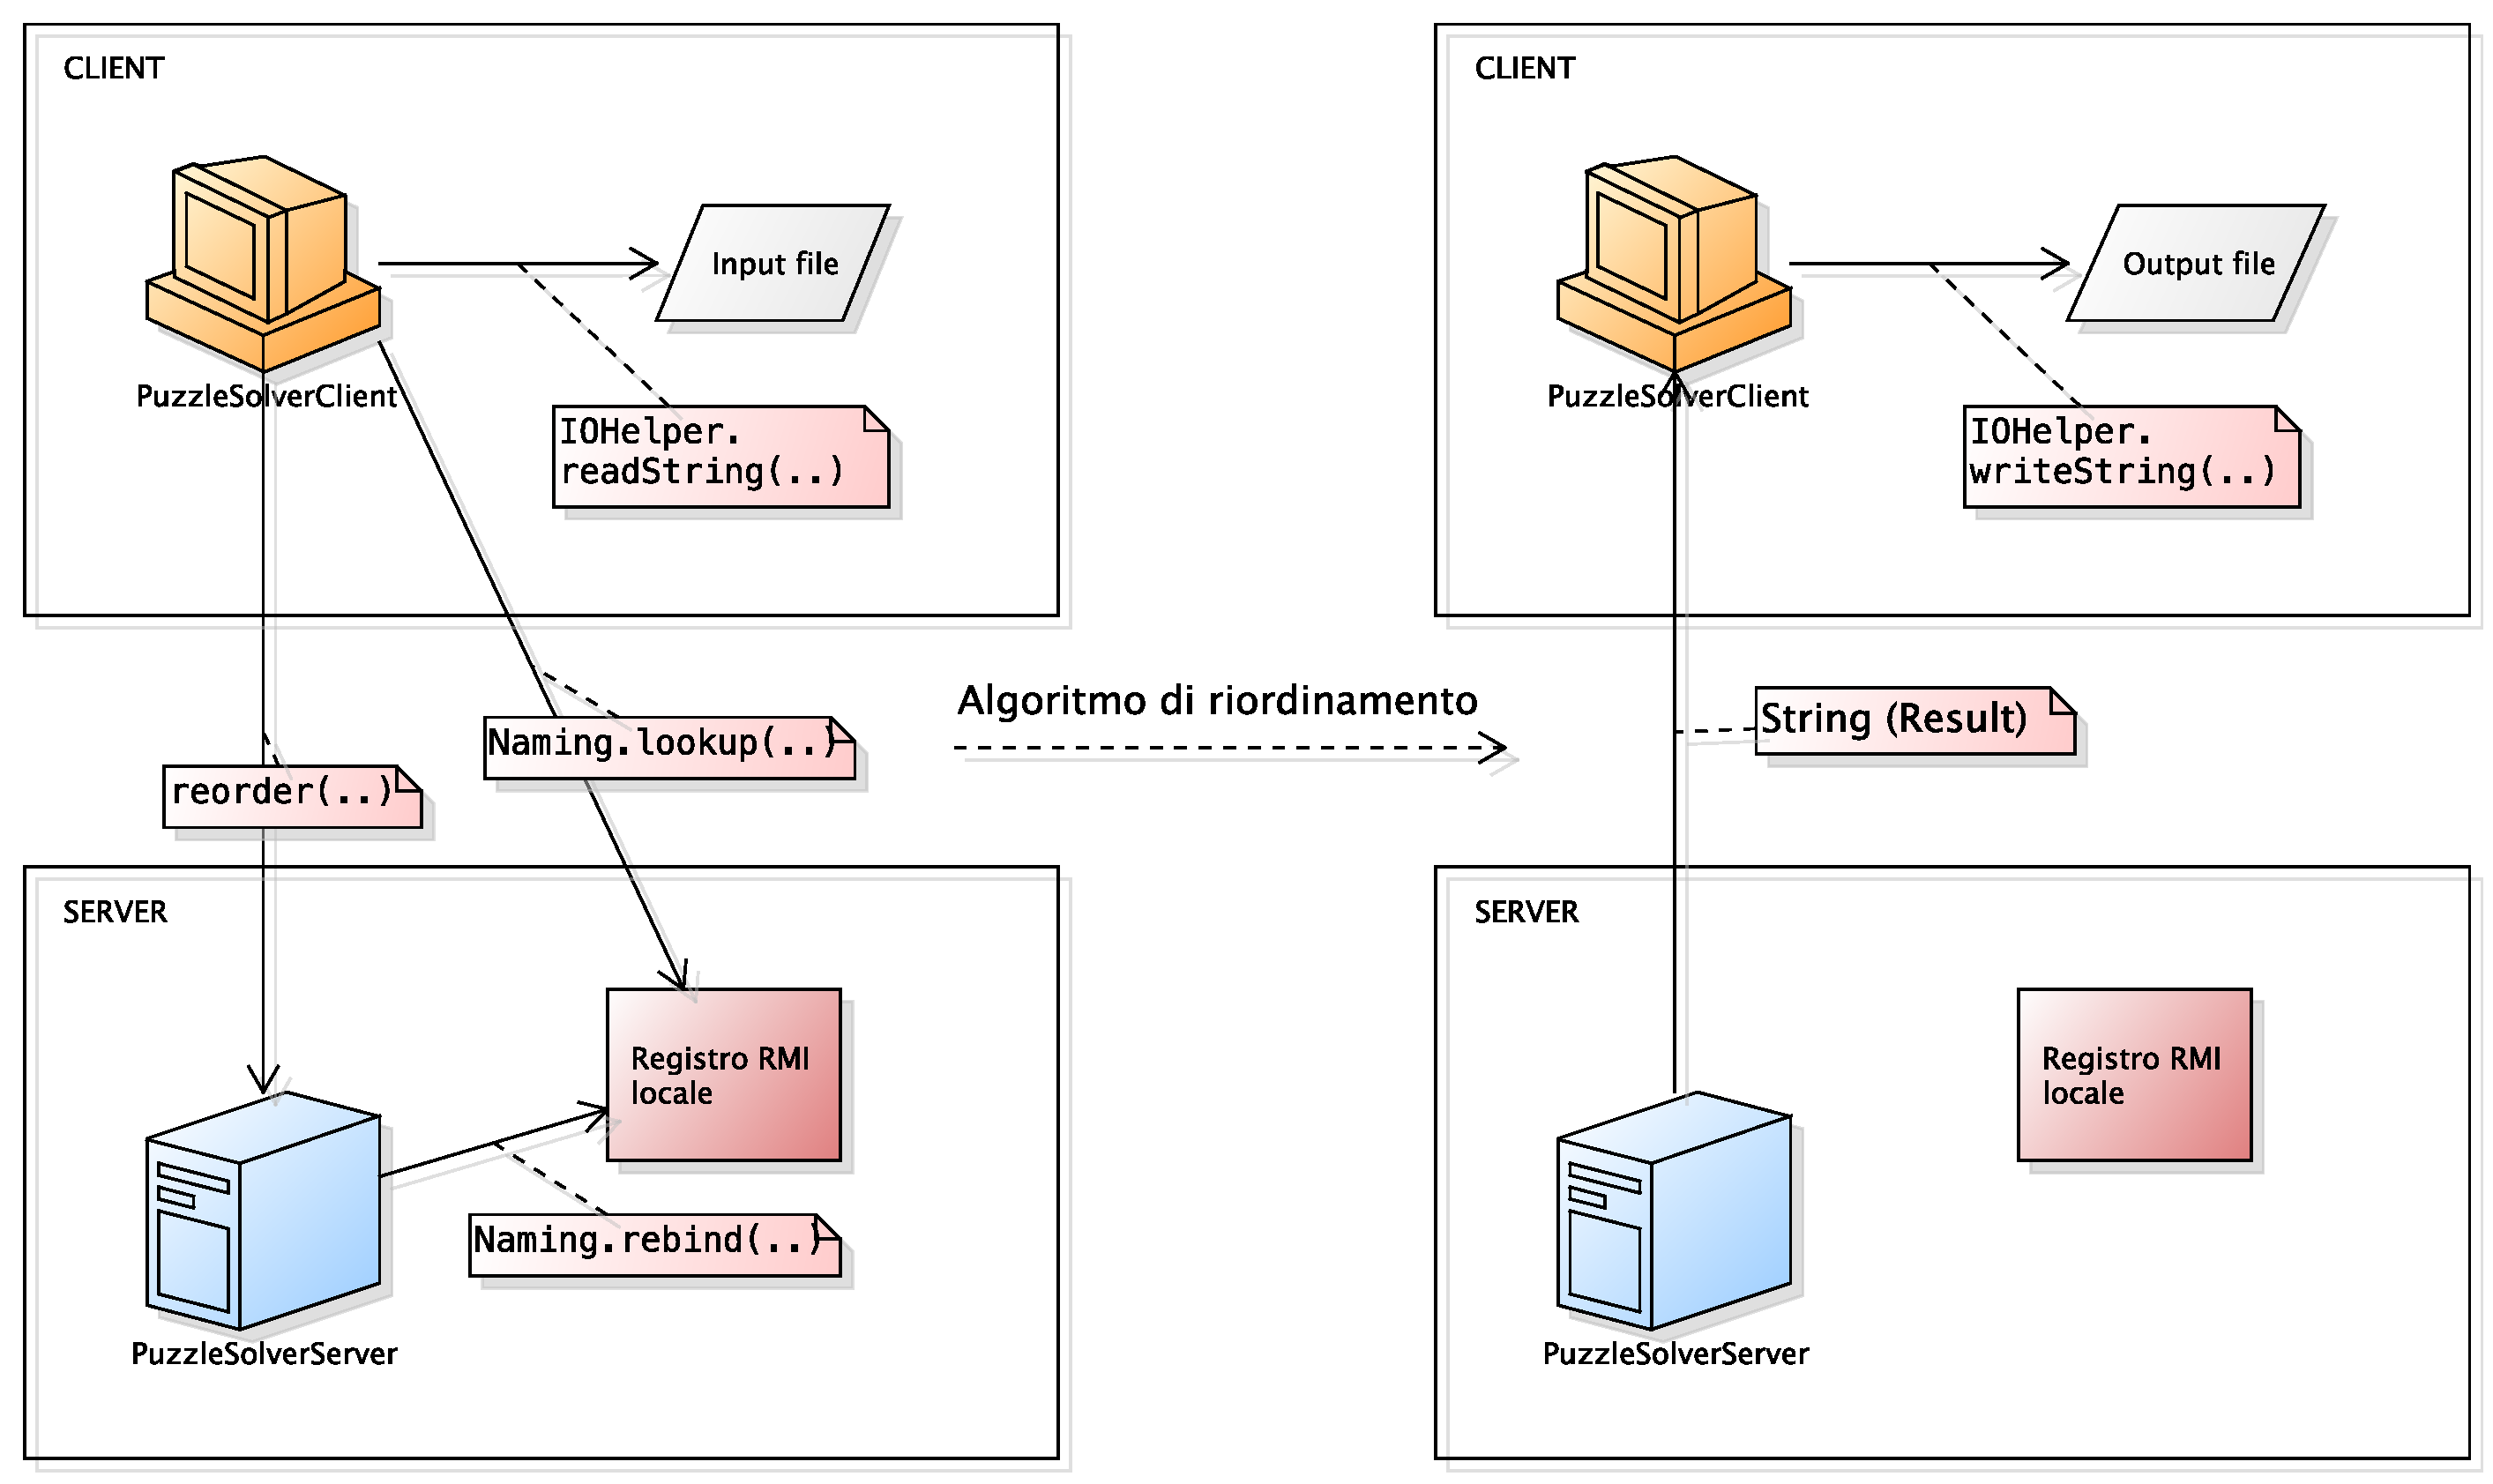
\includegraphics[scale=0.4]{./images/rmi.pdf}}
    \caption{Vista generale implementazione RMI in PuzzleSolver}
\end{figure}

\subsection{L'intefaccia ISolver}

L'interfaccia \texttt{ISolver} estende l'interfaccia \texttt{Remote} che fa da semplice marcatore di tipo
per l'oggetto remoto. \texttt{ISolver} contiene solamente la definizione del metodo remoto \texttt{reoder(String inputPath)},
che sarà implementato dalla classe \texttt{PuzzleSolverServer} con l'algoritmo di risoluzione. Tale metodo, può provocare
un'eccezione di tipo \texttt{RemoteException} a causa di eventiuali problemi di connessione o comunicazione col server.
L'interfaccia è presente sia nel modulo server che nel modulo client, quest'ultimo, infatti, necessita esclusivamente della
definizione del meteodo remoto da invocare visto che non sarà la JVM che risiede nel client ad eseguirlo.


\subsection{La classe PuzzleSolverServer}

L'instanza di questa classe rappresenta l'oggetto remoto il cui riferimento viene reso disponibile al client.
Il \texttt{main} della classe, infatti, crea un oggetto di tipo \texttt{PuzzleSolverServer} e tramite il medoto statico
\texttt{rebind(String uri, Remote obj)} della classe \texttt{Naming} registra l'instanza dell'oggetto creato nel
registro RMI locale. La stringa \texttt{uri}, contenente il nome del server e l'identificativo associato all'oggetto, sarà
utilizzata anche dal client per ottenere il riferimento a tale oggetto.
La classe \texttt{PuzzleSolverServer} espone il metodo remoto \texttt{reorder(String inputPath)} che può essere invocato
da una JVM remota ed esegue l'algoritmo di risoluzione del puzzle. Il metodo è stato dichiarato tramite la keyword
\texttt{synchronized} in modo che il server possa gestire più client in attesa mentre esegue l'algoritmo per il client attivo.
Il metodo \texttt{reset()}, inoltre, assicura che il valore di tutti i campi dati venga risportato a quello originale per
il corretto funzionamento del metodo \texttt{reoder(String inputPath)} invocato dal client sucessivo.


\subsection{La classe PuzzleSolverClient}

La classe \texttt{PuzzleSolverClient}, una volta letto il contenuto dle file di input, si occupa di ottenere un riferimento
all'oggetto instanziato sul server. Questo è possibile tramite il metodo statico \texttt{lookup(String uri)} della classe
\texttt{Naming} che interroga il registro RMI remoto e ottiene il riferimento all'oggetto grazie all'\texttt{uri} identificativo
associato. Inoltre il client, che contiene a sua volta la definizione dell'intefaccia \texttt{ISolver}, può ottenere il
riferimento remoto effettuando un downcast proprio ad un oggetto di tipo \texttt{ISolver}, su cui è possibile invocare il metodo
remoto \texttt{reorder(String inputPath)}.

\end{document}
